%% Paper A — Collective-risk climate dilemma with LLM agents.
%% Royal Society Interface template (rsproca_new, openacc).

\documentclass[openacc]{rsproca_new}

\usepackage[utf8]{inputenc}
\usepackage{eurosym}
\usepackage{newunicodechar}
\newunicodechar{€}{\euro{}}
\usepackage{booktabs}
\usepackage{multirow}

\addbibresource{refs.bib}

\jname{rsif}
\Journal{J R Soc Interface\ }

\begin{document}

\title{Do language-model agents take catastrophe risk seriously? Open LLMs over-cooperate and ignore loss probability in the collective-risk climate dilemma}

\author{Author 1$^{1}$}

\address{$^{1}$Affiliation, City, Country}

\subject{behavioural game theory, artificial intelligence, computational social science}

\keywords{large language models, collective-risk social dilemma, climate cooperation, agent-based modelling, behavioural validity, risk sensitivity}

\corres{Corresponding author\\
\email{tcnguyen2365@gmail.com}}

\begin{abstract}
Large language models are increasingly proposed as drop-in surrogates for human participants, including in social dilemmas where cooperation must be weighed against catastrophe risk. We test this proposal in Milinski's collective-risk dilemma, a climate-protection game in which six players over ten rounds must jointly invest €120 or face a probabilistic loss of all remaining wealth. Across three open instruction-tuned models (Qwen2.5-7B, Gemma-2-9B, Llama-3.1-8B) served on the FAIRGAME framework, agents reach the target on 100\% of games at every loss probability and invest far more than people (final group totals €158--187 versus human €118/€92/€73, against a €240 maximum). Critically, they are insensitive to the very manipulation that governs human behaviour: as catastrophe risk falls from 90\% to 10\%, human investment declines sharply (ANOVA $F=13.78$, $P<0.0001$) whereas models do not ($F=1.76$/$2.23$/$3.64$; equivalence tests bound every model's response below half the human decline). This over-cooperation is a steerable default persona, not a fixed trait: a selfish prompt collapses success to 0--27\% while neutral and cooperative prompts sit at the ceiling. The pattern is largely language-invariant in content, though format compliance degrades for some low-resource pairings. Open LLM agents thus behave as risk-insensitive over-cooperators whose prosociality is a prompt-set knob, and are not behaviourally valid surrogates for studying cooperation under catastrophe risk.
\end{abstract}

\begin{fmtext}
Do language-model agents take catastrophe risk seriously? A growing literature recruits large language models as artificial participants in economic games, treating their choices as proxies for human behaviour \cite{argyle2023out,horton2023llm,aher2023using,park2023generative}. Yet the decisions that matter most for cooperation are those made in the shadow of disaster, where the rational stakes shift with the probability of catastrophe. Milinski's collective-risk social dilemma \cite{milinski2008climate} makes this concrete: groups must collectively fund a climate target or gamble that a wealth-destroying lottery will spare them. In people, lowering the loss probability sharply erodes investment. Here we ask whether open instruction-tuned LLM agents reproduce this hallmark sensitivity, or merely cooperate by reflex. Across three models, five languages and four dispositional prompts, we find the latter: agents secure the target everywhere, indifferent to the risk that drives human players.
\end{fmtext}

\maketitle

\section{Introduction}

Collective-risk social dilemmas distil the central tension of climate cooperation into a tractable laboratory paradigm: a group can avert a shared catastrophe only if its members contribute enough to a common pool, yet each contribution is privately costly and the benefit of averted disaster is non-excludable \cite{milinski2008climate}. This structure is the canonical tragedy of the commons \cite{hardin1968tragedy}, in which individually rational restraint is undersupplied because the returns to cooperation accrue to all while the costs fall on the contributor, and it underlies the broader literature on social dilemmas \cite{dawes1980social} and the chronic under-provision of public goods \cite{ledyard1995public}. What makes the collective-risk dilemma diagnostically powerful, and what distinguishes it from the institutional solutions catalogued by \textcite{ostrom1990governing} and analysed in evolutionary models of institutional incentives for collective-risk games \cite{duong2026cost}, is its manipulation of the loss probability: when the group fails to meet the target, a lottery destroys everyone's remaining endowment with probability $p$, and varying $p$ traces out how much catastrophe risk people are willing to insure against. In \textcite{milinski2008climate}'s experiments human investment falls systematically as the risk of loss recedes, so the response of contributions to the loss-probability manipulation, rather than the mean level of cooperation, is the signature of genuine risk-sensitive decision making. It is precisely this comparative-static response that any behavioural surrogate must reproduce to be considered valid.

A rapidly growing body of work proposes large language models (LLMs) as simulated human subjects, or ``silicon samples'', that might stand in for costly and slow human experimentation \cite{argyle2023out}. Such agents have been used to populate economic and survey settings as homo silicus \cite{horton2023llm}, to instantiate believable interacting personas in generative social simulations \cite{park2023generative}, and to reproduce classic findings from psychology and behavioural economics when prompted to play the role of human participants \cite{aher2023using}. Some studies report that the aggregate distribution of LLM responses can approximate human samples closely enough to pass a behavioural Turing test across a battery of economic games \cite{mei2024turing}. The promise is that, if these systems faithfully mirror human behaviour, they could serve as cheap, scalable pilots for experimental design and even as stand-ins for populations that are difficult to recruit. Mapping where machine behaviour does and does not track human behaviour is, accordingly, central to the emerging social physics of artificial intelligence \cite{han2026socialphysics}. The load-bearing premise, however, is behavioural validity: an LLM is a useful surrogate only insofar as it reproduces not merely plausible average behaviour but the structured way in which human behaviour responds to the experimental levers that define a paradigm.

That premise has rarely been tested against the diagnostic comparative statics of canonical multi-player human experiments. Much existing work evaluates LLMs in two-player matrix games such as the prisoner's dilemma and other repeated interactions \cite{akata2023playing,feng2024survey}, or characterises the strategic dispositions and biases models reveal in simple economic games \cite{brookins2023playing,huynh2025understanding}, and recent audits show that payoff scaling, prompt language and moral framing systematically shape LLM cooperation \cite{huynh2026payoff,buscemi2025communication,backmann2025ethics}. Multi-agent commons settings have also begun to be explored: societies of LLM agents typically fail to sustain a shared resource \cite{piatti2024cooperate} and converge to poor collective outcomes when scaled to hundreds of agents \cite{willis2026collective}; but these designs lack the graded experimental manipulation whose effect on behaviour is the object of validation. Where models are probed more systematically, they are found to exhibit response biases and prompt sensitivities that diverge from human patterns \cite{tjuatja2024llms}, and silicon-sample conclusions can swing with defensible-but-arbitrary analytic choices \cite{cummins2025threat}, raising the question of whether apparent human-likeness survives a manipulation check. Two further gaps compound the problem: studies seldom verify that a model reproduces the direction and magnitude of a key treatment effect, and they seldom test whether whatever behaviour is observed is robust across model families, across the languages in which the task is posed, and across the dispositional framings that ought to move a genuinely human-like agent. Without such robustness probes it is impossible to separate a stable behavioural trait from an artefact of a single model, language, or prompt.

We address this gap with a faithful replication of \textcite{milinski2008climate}'s collective-risk climate dilemma using LLM agents on the FAIRGAME multi-agent framework \cite{fairgame2025}. Six agents, each endowed with €40 over ten rounds, choose in each round to invest €0, €2 or €4 into a shared climate account toward a cumulative group target of €120; if the target is met every player keeps what remains of their endowment, and if it is missed a single group lottery destroys everyone's holdings with probability $p$. We vary the catastrophe risk across treatments, $p \in \{90\%, 50\%, 10\%\}$, exactly as in the human experiments, and cross this manipulation with three open instruction-tuned models (Qwen2.5-7B-Instruct \cite{qwen2025}, Gemma-2-9B-it \cite{gemma2024} and Llama-3.1-8B-Instruct \cite{llama2024}), five languages, and four dispositional prompts (neutral, cooperative, selfish and risk-averse), running ten independent groups per condition. This $3 \times 5 \times 4$ design lets us ask not only whether LLM agents cooperate, but whether their cooperation responds to risk as human cooperation does and whether any such response is robust across models, languages and dispositions.

Our central finding is that these agents are not behaviourally valid surrogates for human cooperation under catastrophe risk. All three models reach the €120 climate target in 100\% of games at every loss probability and invest far more than people, with final group totals of €158--187 against the human €118/€92/€73 (where €240 is the theoretical maximum), so they massively over-cooperate relative to human baselines (table~\ref{tab:baseline}). Decisively, they are insensitive to catastrophe risk: where human investment declines steeply as the loss probability falls (risk ANOVA $F = 13.78$, $P < 0.0001$), the models' cumulative trajectories nearly coincide across risk levels and the manipulation has no comparable effect ($F = 1.76$, $2.23$ and $3.64$; figure~\ref{fig:risk}). This over-cooperation is not a fixed trait but a steerable default persona: a selfish disposition prompt collapses target success to 0\% for Qwen and Gemma and 27\% for Llama, a risk-averse prompt yields intermediate success (73--93\%), and the neutral and cooperative framings sit at the ceiling, while the pattern is broadly language-invariant in content even as format compliance degrades sharply for some low-resource pairings (figure~\ref{fig:moderators}). The contributions of this paper are thus threefold: a faithful, multi-condition replication of a canonical collective-risk experiment with LLM agents; quantitative evidence that open models act as risk-insensitive over-cooperators whose prosociality is a prompt-set knob rather than a property of the strategic situation; and, on this basis, an explicit validity criterion for the use of LLMs as silicon samples, namely that the appropriate test is the agents' response to the risk manipulation, not the mean level of cooperation they happen to display.

%% Methods + Results + floats for the CRSD paper (\input by main.tex).

\section{Methods}

\subsection{The collective-risk climate dilemma}
We replicate the collective-risk social dilemma (CRSD) of \textcite{milinski2008climate}. Six players each receive a private endowment of €40 and play ten rounds. In every round each player simultaneously and privately invests €0, €2 or €4 into a shared climate account; the climate cover story matches the original. The group must accumulate a cumulative target of €120 across all players and rounds. If the target is reached, each player keeps €40 minus their own total investment; if it is missed, a single group-level lottery is drawn in which, with loss probability $p$, every player loses everything (final payoff €0), and otherwise each keeps their remainder. The catastrophe risk $p$ is crossed at three levels, $p\in\{90\%,50\%,10\%\}$, which constitutes the diagnostic manipulation of the design. There is no communication. Faithful to the original ``took notes by hand'' visibility, players observe one another's per-round contributions under fixed anonymous identifiers but are never shown the running cumulative total; the maximum attainable group total is €240 (six players each investing €4 in all ten rounds), twice the target. We run ten independent groups per cell.

\subsection{Agents, models and protocol}
Each agent is an instruction-tuned LLM that receives a single natural-language prompt comprising a brief of the game rules, the history of play so far, and a disposition block, after which it reasons briefly and emits a parseable decision line of the form \texttt{CONTRIBUTION = X} (with $X$ one of 0, 2 or 4). Within each round, all six agents' decisions are collected in a single lockstep batch so that play is genuinely simultaneous. The protocol is built on the FAIRGAME multi-agent framework \parencite{fairgame2025}. We serve three open-weight instruction-tuned models, Qwen2.5-7B-Instruct \parencite{qwen2025}, Gemma-2-9B-it \parencite{gemma2024} and Llama-3.1-8B-Instruct \parencite{llama2024}, via vLLM at temperature 0.8 with a fixed seed to make runs reproducible; all simulations were executed offline on a single RTX PRO 6000. Exact model identifiers, decoding settings and per-condition game counts are listed in the electronic supplementary material. We cross the game with five languages (English, French, Arabic, Chinese, Vietnamese) and four dispositional prompts (neutral, cooperative, selfish, risk-averse), each rendered as a short instruction prepended to the brief (the neutral prompt adds no disposition).

\subsection{Measures and analysis}
For each game we record whether the €120 target was reached (success), the final group total, and the number of ``fair-sharers'' per group, defined as players whose total contribution is at least €2 per round on average (i.e.\ at least €20 over the ten rounds), matching Milinski's notion of a fair share. The central diagnostic is the model's sensitivity to the loss-probability manipulation, which we test with a one-way ANOVA of the final group total across the three treatments, computed separately per model and benchmarked against the human ANOVA ($F=13.78$, $P<0.0001$); model success rates are compared with the human baseline using Fisher's exact test and group totals using Welch's $t$-test. Each significance test is accompanied by a bias-corrected effect size (Hedges $g$ for the mean contrasts) with 95\%\ confidence intervals, and the family-wise error rate across the nine baseline cells is controlled with the Holm--Bonferroni procedure; the full effect-size tables appear in the electronic supplementary material. Throughout, we log the \texttt{parse\_fallback} (format non-compliance) rate for every cell and report it as a joint data-quality and fairness signal, since it varies systematically across languages. Finally, because agents are shown each player's per-round contributions but never the running cumulative total, any apparent target tracking must arise from the model's own arithmetic self-summation across the visible history rather than from a displayed total; we treat this requirement as a caveat when interpreting the models' near-uniform attainment of the target.

\section{Results}

\begin{table*}[t]
\caption{Behaviour of the three LLM agents in the faithful baseline (English
prompt, neutral disposition) against the human benchmark of Milinski
\textit{et al.}\ \cite{milinski2008climate}, by loss probability. ``Target
reached'' is the fraction of the ten groups whose cumulative investment met the
€120 threshold; ``Final total'' is the mean group investment ($\pm$ s.e.m.);
``Fair-sharers'' is the mean number of group members (of six) investing at least
€2 per round on average. All LLM-versus-human contrasts are significant (Welch
$t$ on totals and Fisher exact on success, all $p<0.05$).}
\label{tab:baseline}
\centering
\begin{tabular}{llccc}
\toprule
Loss prob. & Player & Target reached & Final total (€) & Fair-sharers \\
\midrule
\multirow{4}{*}{90\%}
 & Human \cite{milinski2008climate} & 50\%  & 118.2 & 3.3 \\
 & Qwen2.5-7B   & 100\% & 183.0 $\pm$ 2.1 & 6.0 \\
 & Gemma-2-9B   & 100\% & 168.2 $\pm$ 3.3 & 5.8 \\
 & Llama-3.1-8B & 100\% & 177.4 $\pm$ 2.9 & 5.8 \\
\midrule
\multirow{4}{*}{50\%}
 & Human \cite{milinski2008climate} & 10\%  & 92.2  & 2.1 \\
 & Qwen2.5-7B   & 100\% & 186.6 $\pm$ 1.2 & 6.0 \\
 & Gemma-2-9B   & 100\% & 162.8 $\pm$ 2.9 & 5.9 \\
 & Llama-3.1-8B & 100\% & 165.2 $\pm$ 3.6 & 5.6 \\
\midrule
\multirow{4}{*}{10\%}
 & Human \cite{milinski2008climate} & 0\%   & 73.0  & 1.1 \\
 & Qwen2.5-7B   & 100\% & 181.0 $\pm$ 2.8 & 5.9 \\
 & Gemma-2-9B   & 100\% & 158.0 $\pm$ 3.9 & 5.8 \\
 & Llama-3.1-8B & 100\% & 170.0 $\pm$ 3.1 & 5.7 \\
\bottomrule
\end{tabular}
\end{table*}

\begin{figure*}[t]
\centering
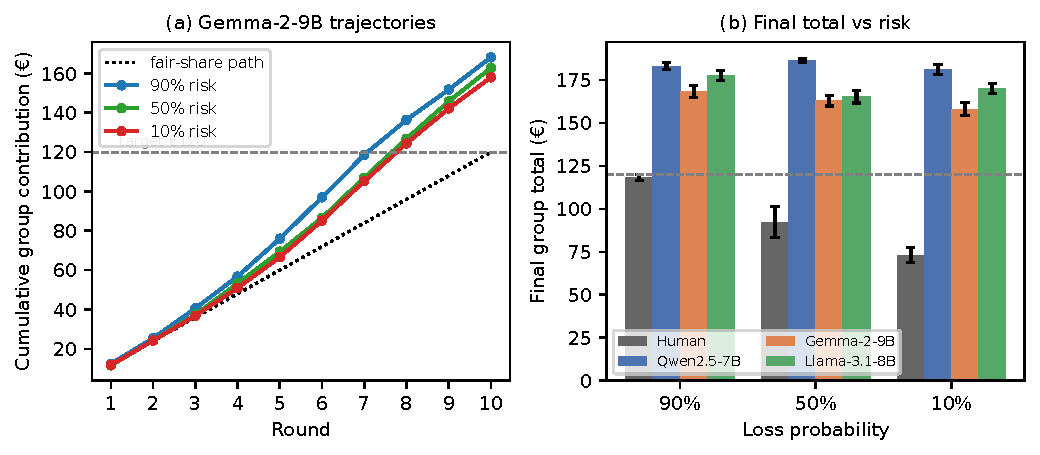
\includegraphics[width=\textwidth]{figures/fig1_risk.pdf}
\caption{Over-cooperation and insensitivity to catastrophe risk.
(\textit{a}) Cumulative group investment per round for Gemma-2-9B at the three
loss probabilities, against the fair-share path and the €120 target; the three
risk curves nearly coincide and all cross the target. (\textit{b}) Final group
total by loss probability for humans \cite{milinski2008climate} and the three
LLMs: humans fall steeply as catastrophe risk declines (one-way ANOVA
$F=13.78$, $p<0.0001$), whereas every model stays flat and far above target
(model ANOVA $F=1.76$/$2.23$/$3.64$). Error bars are s.e.m.}
\label{fig:risk}
\end{figure*}

In the human collective-risk dilemma, the loss probability is the lever that separates prudent from reckless groups: only half of Milinski's groups reached the €120 climate target under the gravest 90\% catastrophe risk, one in ten reached it at 50\%, and none reached it at 10\%, with final group totals falling from €118 through €92 to €73 as the threat receded \cite{milinski2008climate}. The LLM agents show no such restraint. In the English, neutral baseline, all three models---Qwen2.5-7B-Instruct, Gemma-2-9B-it and Llama-3.1-8B-Instruct---reach the target on 100\% of games at every loss probability (table~\ref{tab:baseline}), and they do so by over-investing rather than by tracking the threat: final group totals cluster between roughly €158 and €187, some 70--78\% of the €240 ceiling attainable if every player invested the maximum in every round, and far above the human totals of €118, €92 and €73. The same over-supply is visible in the count of ``fair-sharers'': where human groups typically contained only one to three players investing at least €20 over the game, the model groups contain roughly six of six. Welch tests on final totals and Fisher exact tests on success counts confirm that these model--human gaps are statistically significant across the board (table~\ref{tab:baseline}).

The decisive diagnostic, however, is not the level of cooperation but its insensitivity to risk. In humans the loss-probability manipulation is what drives behaviour, producing a steep and monotone decline (one-way ANOVA across the three treatments $F=13.78$, $P<0.0001$). The models reproduce none of this gradient: the analogous ANOVA on final group totals yields only $F=1.76$ ($P=0.19$) for Qwen, $F=2.23$ ($P=0.13$) for Gemma and $F=3.64$ ($P=0.040$) for Llama, and even the lone nominally significant case is weak and non-monotone rather than the orderly human descent. Figure~\ref{fig:risk}a makes the failure concrete: the cumulative-contribution trajectories for 90\%, 50\% and 10\% loss risk nearly coincide and all cross the €120 target well before the final round, regardless of how much is actually at stake. Figure~\ref{fig:risk}b sharpens the contrast by plotting final total against loss probability: the human line falls steeply as catastrophe risk recedes, whereas all three model lines stay essentially flat and far above target. The manipulation that makes the experiment informative about human risk preferences leaves the models almost untouched.

\begin{figure*}[t]
\centering
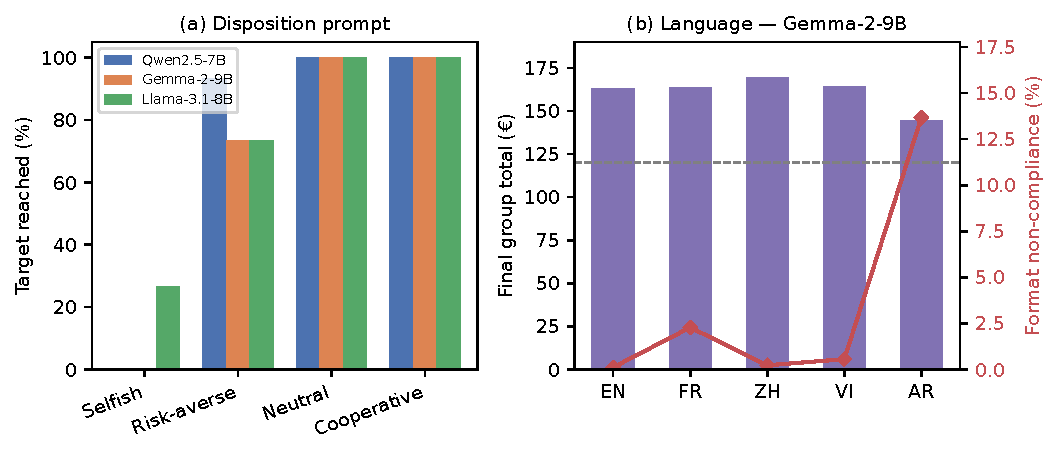
\includegraphics[width=\textwidth]{figures/fig2_moderators.pdf}
\caption{Moderators of the over-cooperation result. (\textit{a}) Target-success
rate by dispositional prompt: a ``selfish'' instruction collapses cooperation
(0\% success for Qwen and Gemma), ``risk-averse'' is intermediate, and
``neutral''/``cooperative'' sit at the ceiling, showing that the default
high-prosociality behaviour is a steerable knob. (\textit{b}) Gemma-2-9B final
total (bars) and format non-compliance rate (line) by prompt language:
cooperation is broadly language-invariant in content, but format reliability
degrades sharply in Arabic.}
\label{fig:moderators}
\end{figure*}

That the default behaviour is a high-prosociality persona rather than a fixed trait becomes clear once disposition is varied. The dispositional prompt is a powerful lever on the same models (figure~\ref{fig:moderators}a): switching the agents from neutral to a selfish disposition collapses target success from the ceiling to 0\% for Qwen and Gemma and to 27\% for Llama, with final group totals dropping into the €33--113 range and many groups now missing the target outright. A risk-averse disposition produces an intermediate regime (success between 73\% and 93\%), while the neutral and cooperative prompts both sit at or near the 100\% ceiling. The behaviour therefore moves across almost the entire feasible range under prompt control, which indicates that the over-cooperative baseline reflects a steerable default persona rather than an immovable property of the architecture---a knob, not a trait.

Finally, the core result is robust across languages while exposing a low-resource fragility that is a fairness caveat rather than an explanation. Translating the game into French, Chinese, Vietnamese and Arabic leaves the substantive outcomes roughly invariant: the models still over-cooperate and still ignore the risk gradient. What does vary is format compliance. The rate of format non-compliance (parse-fallback) stays below 2.5\% in most cells but spikes to 13.7\% for Gemma in Arabic and 14.8\% for Llama in Vietnamese (figure~\ref{fig:moderators}b), a non-trivial degradation that the framework logs as a data-quality and fairness signal. Crucially, the English baseline that carries the over-cooperation result has a parse-fallback rate of essentially 0\%, so the failure to track risk cannot be dismissed as an arithmetic or parsing artefact: the models read the game correctly and still pour in resources regardless of the odds.


\section{Discussion}

Our results converge on a single, compact characterisation of how these open instruction-tuned agents play Milinski's collective-risk climate dilemma: they are risk-insensitive, prompt-steerable over-cooperators. Each of the three threads of evidence---the elevated level of cooperation, its near-total decoupling from catastrophe risk, and its responsiveness to dispositional framing---constrains the interpretation of the others, and only together do they delineate the behavioural surface we observe.

The first and most immediate finding is over-cooperation. Across all three models, the €120 climate target is reached in 100\% of games at every loss probability, with final group totals of €158--187 against the €240 theoretical maximum (table~\ref{tab:baseline}). Human groups in the same game, by contrast, reach the target only intermittently and invest substantially less---€118, €92 and €73 as the loss probability falls from 90\% to 50\% to 10\% \cite{milinski2008climate}. The agents thus sit far above the human band at every level of risk, sustaining group investment that no human cohort in the original experiment approached. Taken in isolation, one might read this simply as a quantitative shift---agents that are more generous than people---and conclude that LLMs are usable but optimistic surrogates whose levels merely require recalibration.

The second finding forecloses that reading. The defining feature of the human collective-risk dilemma is that cooperation tracks the probability of catastrophe: people invest more when the danger of losing everything is high and visibly retreat as that danger recedes, a decline that is large and highly reliable (risk ANOVA $F=13.78$, $P<0.0001$) \cite{milinski2008climate}. The agents show essentially none of this structure. Their cumulative trajectories across the three risk treatments nearly coincide (figure~\ref{fig:risk}), and the corresponding risk effects are weak and inconsistent ($F=1.76$, $2.23$ and $3.64$ across the three models), several-fold below the human effect. Equivalence and Bayes-factor analyses sharpen this null into positive evidence: every model's 90\%-to-10\% response is statistically equivalent to less than half the human decline, and the Bayes factors favour the no-effect null for two of the three models (electronic supplementary material, table~S3). This is the decisive result. The over-cooperation is not a generous version of human play; it is play that lacks the very dependency on which the dilemma turns. The agents reach the target not because they have weighed a high risk of ruin and responded to it, but because they cooperate at a high fixed level regardless of whether the risk is severe or slight. What looks like a behavioural surface resembling human cooperation is therefore missing the human risk-preference structure underneath it. This echoes prospect-theoretic audits of frontier models, which find systematically distorted probability weighting in LLM decision making under uncertainty \cite{jia2024decision} and only unreliable, persona-dependent control over their economic risk attitudes \cite{liu2025aligning}.

The third finding shows that this surface is not a fixed trait but a default persona that the prompt can move at will. Holding the game constant and varying only the dispositional block, target success collapses from the ceiling to 0\% for Qwen and Gemma and to 27\% for Llama under a selfish disposition, sits at an intermediate 73--93\% under a risk-averse framing, and returns to the ceiling under neutral and cooperative framings (figure~\ref{fig:moderators}). The prosociality we observe at baseline is thus a knob, not a constant: a single sentence of role specification spans nearly the entire range from defection to full cooperation. The agents are steerable, and the steering operates on disposition---on who the model is told to be---rather than on the material incentive that the risk manipulation alters. This is the mirror image of the human result, in which the incentive moves behaviour and the framing is comparatively inert.

The fourth thread establishes that this picture is a property of the agents rather than of the language in which they are tested. The over-cooperation, the risk insensitivity and the dispositional steerability reproduce in substance across the five languages: the content of play is broadly language-invariant. Where languages differ is in format compliance rather than in cooperative behaviour. Some low-resource model--language pairings degrade sharply---Gemma in Arabic and Llama in Vietnamese reach non-compliance rates of 13.7\% and 14.8\%, respectively---while the English baseline parses at essentially 0\% failure (figure~\ref{fig:moderators}). Because the over-cooperation is already saturated in the clean English condition, it cannot be an artefact of parsing fallback, and the cross-language degradation is best read as a separate fairness signal about uneven instruction-following rather than as a modifier of the cooperative result, in line with the language-driven biases documented in other multi-agent LLM settings \cite{buscemi2025communication,huynh2026payoff}.

Synthesising these threads, the behaviour of these agents is well described as a risk-insensitive, prompt-steerable over-cooperator: a system that produces the outward form of cooperative climate action---reaching the target, sharing the burden---while lacking the internal coupling to catastrophe risk that, in humans, generates that action and modulates its intensity. The cooperation is real as output and absent as mechanism. This distinction matters directly for the growing programme that proposes to use LLMs as ``silicon subjects'' standing in for human participants in social-scientific experiments \cite{argyle2023out,horton2023llm}. That programme's appeal rests on the assumption that a model trained on human text reproduces not just human-sounding responses but human response \emph{functions}---the way behaviour changes as the experimenter changes the situation. Our findings caution that the two can come apart precisely where it matters. An investigator who validated these agents on mean cooperation alone would find them strikingly human-compatible, even generous; an investigator who validated them on the treatment effect---the response to the manipulation that defines the paradigm---would find them inert. The correct validity test for a silicon subject is therefore not whether it reproduces the level of a behaviour but whether it reproduces the behaviour's dependence on the experimental variable of interest, and on that test these agents fail the collective-risk dilemma. This criterion aligns with recent calls to validate LLM simulations statistically against human data rather than by surface plausibility \cite{hullman2026validating,cummins2025threat}. A companion study applies the same criterion to a different institution---costly peer punishment in the public-goods game---and finds the complementary dissociation: the behaviour is reproduced while its institutional function and cross-cultural structure are not \cite{companionPGG2026}.

The implication for climate-cooperation modelling is correspondingly specific. The collective-risk game was designed to capture the strategic core of climate negotiation---the choice to invest now against an uncertain future catastrophe whose probability is the very quantity at stake \cite{milinski2008climate}. An agent population that invests heavily but ignores the catastrophe probability will, if used to simulate such negotiations, systematically misrepresent the comparative statics that policy cares about: it will predict robust cooperation where humans would defect as perceived risk falls, and it will be unresponsive to interventions that work by changing risk perception. Such agents may still be useful as configurable populations whose disposition is set deliberately rather than discovered---indeed, deliberately designed artificial players can themselves steer cooperation in mixed human--machine interactions \cite{zimmaro2024discriminatory}---but they are not instruments for reading off how risk shapes collective action.

\subsection{Limitations}

Several constraints bound these conclusions. First, the study examines three open instruction-tuned models in the 7--9B parameter range, served at a single decoding temperature. We cannot say from these data whether the risk insensitivity is a property of scale, of open versus frontier training, or of the temperature regime; larger or differently aligned models may recover some sensitivity to the loss probability, and our claims are properly scoped to the class of models tested rather than to LLM agents in general.

Second, the design follows Milinski in withholding the running cumulative total, so an agent that responds to remaining distance from the €120 target must compute that total itself by summing the per-round contributions it has been shown. This faithful no-running-total design introduces a self-summation confound: an agent that fails to track the target arithmetically would be unable to modulate investment as the target approached, and some of the observed flatness could in principle reflect arithmetic limitation rather than genuine risk insensitivity. We regard this as mitigated rather than eliminated. The near-zero English parse-failure rate shows the models reliably produce well-formed decisions, and the risk manipulation does not change the arithmetic burden---the summation task is identical across loss probabilities---so a purely arithmetic account cannot explain why behaviour fails to differ \emph{between} risk treatments, which is the effect of interest. Nonetheless we acknowledge the confound, and isolating risk response from running-total computation is a target for future designs.

Third, the cross-language results carry a confound of their own. Format non-compliance is unevenly distributed across model--language pairings, and although we interpret over-cooperation as language-invariant because it saturates in the clean English condition, the elevated fallback rates in some low-resource pairings mean that the behavioural samples in those cells are smaller and potentially non-random. We have treated this non-compliance as a fairness signal about uneven instruction-following, but it remains a limitation on the precision of the cross-language comparison.

Fourth, the behaviour is demonstrably prompt-sensitive, which cuts two ways. It is substantively part of our result---steerability is a finding---but it also means that the specific levels we report are tied to the particular game brief and dispositional wordings we used, and different but equally reasonable phrasings could shift the baseline within the range the disposition sweep maps out. Finally, the over-cooperation we observe is very likely inflated by alignment training: instruction tuning and preference optimisation explicitly reward helpful, prosocial, cooperative outputs, so a default persona that cooperates strongly is the expected consequence of the training objective rather than an emergent strategic disposition, and this provides a parsimonious account of why the baseline sits so far above the human band.

\section{Conclusion}

In Milinski's collective-risk climate dilemma, open instruction-tuned LLM agents reach the cooperative target on 100\% of games at every level of catastrophe risk, investing well above human levels, and---decisively---show essentially none of the steep, reliable decline in cooperation that humans exhibit as the probability of catastrophe falls. The behaviour that governs human play, the response to risk, is the behaviour these agents lack; what they retain is a high, fixed propensity to cooperate that a single dispositional sentence can drive from full cooperation to outright defection. These agents are best understood as risk-insensitive, prompt-steerable over-cooperators: they reproduce the surface of cooperative climate action without the underlying human risk-preference structure that produces it. The consequence for using LLMs as silicon subjects is sharp. Their behaviour is governed by manipulation of the prompt, not by the mean incentives of the game---it is controlled by what the model is told to be, not by what the situation rewards---so the meaningful test of behavioural validity is the response to the experimental manipulation, not the average level of cooperation. On that test, in the dilemma that most directly models climate cooperation, these agents do not yet stand in for people.

\enlargethispage{20pt}

\ethics{This study involved no human or animal participants. All behavioural data were generated by computational simulations of large language models and therefore required no ethics approval.}

\dataccess{All materials needed to reproduce the study---the FAIRGAME-based simulation code, the prompt templates in five languages, the configuration files, the per-game result files for all three models, and the analysis script (\texttt{analysis/analyze.py}) that regenerates every figure, table and number---together with the electronic supplementary material are available in the project repository and will be deposited with a permanent DOI (Zenodo) on acceptance [DOI to be inserted]. The human benchmark is taken from the published data of Milinski \textit{et al.}\ \cite{milinski2008climate}.}

\aucontribute{Author~1: conceptualization, methodology, software, formal analysis, investigation, data curation, visualization, and writing (original draft, review and editing). The author gave final approval for publication and agrees to be held accountable for the work performed therein.}

\competing{The author(s) declare that they have no competing interests.}

\funding{This research received no specific grant from any funding agency in the public, commercial or not-for-profit sectors.}

\ack{We thank the developers of the FAIRGAME framework and of the vLLM inference engine. The simulations used the Qwen2.5, Gemma~2 and Llama~3.1 open-weight models.}

\disclaimer{Large language models were used solely as the objects of study (the simulated agents); all analysis, figures and text were produced and verified by the authors.}

\printbibliography

\end{document}
